\part{Modello di prova d'esame - Semaforo \emph{mutex}}

\small
\begin{framed}
	\noindent Un {\tt mutex} \`e un tipo particolare di semaforo che pu\`o assumere soltanto
	due stati: libero oppure occupato.  Inoltre, un mutex ricorda l'identit\`a del
	processo che lo ha occupato. \`E un errore se lo stesso processo tenta di
	occupare nuovamente il mutex prima di averlo liberato. Inoltre, \`e un errore
	se il mutex viene liberato da un processo diverso da quello che lo aveva
	occupato.\\\\Per realizzare un mutex definiamo la seguente struttura (file {\tt sistema.cpp}):
	
	\begin{verbatim}
		struct des_mutex {
			natl owner;
			des_proc* waiting;
		};
	\end{verbatim}
	\noindent Se il mutex \`e occupato, il campo {\tt owner} contiene l'id del processo che
	lo ha occupato, altrimenti {\tt owner} vale 0.  Il campo {\tt waiting} serve a
	realizzare una lista di processi in attesa di acquisire il {\tt mutex}.\\\\Le seguenti primitive, accessibili dal livello utente, operano sui {\tt mutex}:
	\begin{itemize}
		\item \verb|natl mutex_ini()| (gi\`a realizzata): inizializza
		un nuovo mutex, con i campi {\tt owner} e {\tt waiting} entrambi a 0, e ne
		restituisce l'identificatore. Se non \`e possibile creare un nuovo mutex
		restituisce {\tt 0xFFFFFFFF}.
		\item \verb|void mutex_wait(natl mux)|: tenta di occupare il
		mutex di identificatore {\tt mux}.  Se il mutex \`e gi\`a occupato sospende il
		processo in attesa che il mutex venga prima liberato.  Abortisce il processo in
		caso di errore.
		\item \verb|void mutex_signal(natl mux)|: libera il mutex di
		identificatore {\tt mux}.  Se qualche altro processo era in attesa, lo
		risveglia e gli cede il mutex (che in questo caso resta occupato). Gestisce una
		eventuale {\em preemption}.  Abortisce il processo in caso di errore.
	\end{itemize}
	\noindent Modificare i file \verb|sistema.cpp| e \verb|sistema.s| in modo da realizzare
	le primitive mancanti.\end{framed}
\normalsize 
\begin{itemize}
	\item I semafori sono primitive generiche che permettono di risolvere una grande varietà di problemi. L'esercizio introduce una nuova tipologia di semaforo, specializzato su alcuni aspetti rispetto ai classici semafori (per esempio potrei concentrarmi sulla questione della mutua esclusione): il \emph{mutex}.
	\item Il semaforo \emph{mutex} presenta solo due stati: libero e occupato. Le proprietà del \emph{mutex} sono indicate nella consegna.
\end{itemize}

\section*{Struttura di una prova d'esame}
\begin{itemize}
	\item \textbf{Unzip della prova d'esame}.
	
	La prima cosa che facciamo è l'unzip del file contenente il codice del nucleo
	\begin{verbatim}
		unzip es1.zip
	\end{verbatim}
	
	\begin{center}
		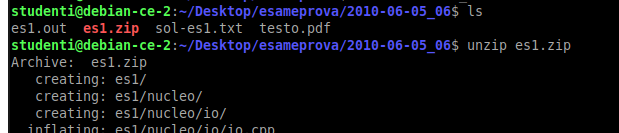
\includegraphics[scale=.9]{img/202.PNG}
	\end{center}
	verrà creata una cartella nella directory in cui ci troviamo. La versione del nucleo offerta è modificata apposta per l'esercizio.
	\begin{multicols}{2}
		\item \textbf{Modifiche del nucleo introdotte per la prova}. 
		
		Le parti aggiunte, così come le aree dove dobbiamo scrivere qualcosa, vengono segnalate con del testo. Ricordarsi che per ricercare testo all'interno dell'editor basta premere lo slash e scrivere quanto desiderato (quando si trova il punto premiamo invio, la ricerca si chiude e possiamo lavorare nel luogo desiderato).
		\columnbreak
		\begin{center}
			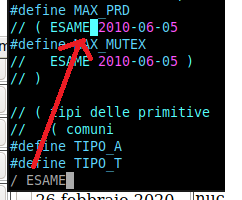
\includegraphics[scale=.9]{img/201.PNG}
		\end{center}
	\end{multicols}
	\item In questo esercizio abbiamo
	\begin{itemize}
		\item Aggiunta di costanti in \emph{include/costanti.h}
		\begin{center}
			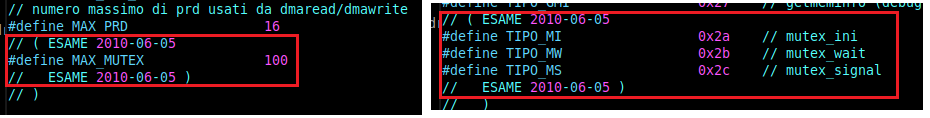
\includegraphics[scale=.8]{img/199.PNG}
		\end{center}
		\item Creazione di un gate in \emph{sistema/sistema.s}
		\begin{center}
			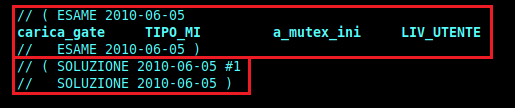
\includegraphics[scale=.9]{img/204.PNG}
		\end{center}
		Abbiamo anche la parte relativa all'assembler dell'unica primitiva implementata.
		\begin{center}
			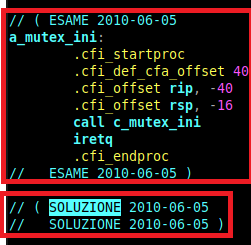
\includegraphics[scale=.9]{img/205.PNG}
		\end{center}
		Si osservino le scritte \emph{SOLUZIONE}: \textbf{tra le due scritte deve essere posto del codice, per forza}. 
		\item \textbf{Strutture dati e implementazione della \emph{mutex$\_$ini}}. 
		
		In \emph{sistema.cpp} abbiamo l'implementazione delle strutture dati necessarie e dell'unica primitiva implementata
		\begin{center}
			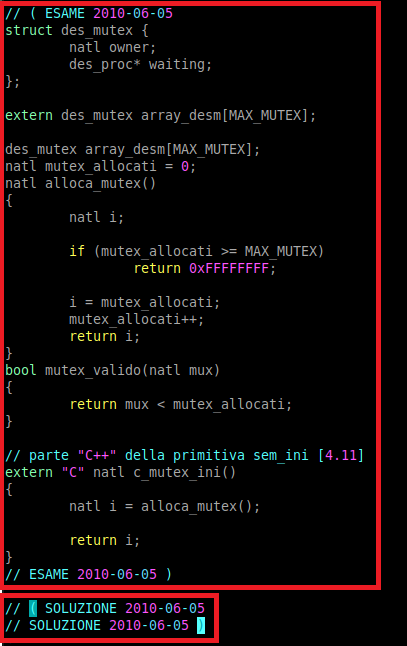
\includegraphics[scale=.9]{img/206.PNG}
		\end{center}
	\end{itemize}
	Per quanto riguarda questo esercizio sono state introdotte delle costanti in \emph{costanti.h}, posto il gate relativo all'unica primitiva realizzata in \emph{sistema.s}. 
	\item \textbf{Programma per la verifica della correttezza del codice}. 
	
	Nella cartella \emph{prog}, in \emph{utente}, è presente un programma che prova ad usare le primitive richieste. Questo programma stampa l'output che ogni prova deve rispettare nel portale di autocorrezione.
	\begin{center}
		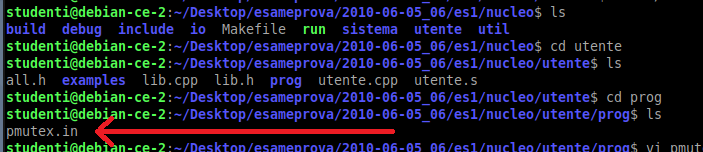
\includegraphics{img/207.PNG}
	\end{center}
	Solitamente il programma cerca sempre di utilizzare le primitive in modo sbagliato, per verificare se abbiamo posto nel codice tutti i controlli richiesti dalla consegna. Si consideri che l'output corretto non garantisce al 100\% che abbiamo svolto l'esercizio correttamente.
\end{itemize}
\section*{Soluzione}
Analizziamo la soluzione
\begin{itemize} 
	\item \textbf{Per quanto riguarda la parte assembler in \emph{sistema.s} abbiamo }
	\begin{verbatim}
		// ( SOLUZIONE 2010-06-05 #1
		carica_gate	TIPO_MW		a_mutex_wait	LIV_UTENTE
		carica_gate	TIPO_MS		a_mutex_signal	LIV_UTENTE
		//   SOLUZIONE 2010-06-05 )
		
		// ( SOLUZIONE 2010-06-05
		a_mutex_wait:
		.cfi_startproc
		.cfi_def_cfa_offset 40
		.cfi_offset rip, -40
		.cfi_offset rsp, -16
		call salva_stato
		call c_mutex_wait
		call carica_stato
		iretq
		.cfi_endproc
		
		a_mutex_signal:
		.cfi_startproc
		.cfi_def_cfa_offset 40
		.cfi_offset rip, -40
		.cfi_offset rsp, -16
		call salva_stato
		call c_mutex_signal
		call carica_stato
		iretq
		.cfi_endproc
		//   SOLUZIONE 2010-06-05 )
	\end{verbatim}
	\begin{itemize}
		\item Poniamo i gate per le primitive che la consegna ci richiede di implementare. Per fare ciò ricorriamo alle nuove costanti poste in \emph{costanti.h} (\emph{TIPO$\_$MW} e \emph{TIPO$\_$MS}). Il livello di privilegio richiesto per attraversare il gate non può che essere \emph{LIV$\_$UTENTE} (l'utente non potrebbe utilizzare le primitive con livello di privilegio maggiore).
		\item Il codice rimanente consiste nell'implementazione della parte Assembler delle primitive. La struttura può essere copiata dalle altre primitive comuni senza grossi problemi (attenzione a cosa stiamo implementando, in esercizi di tipologia diversa il contenuto di questa parte potrebbe cambiare).
		
		\textbf{Attenzione a una cosa}: non si rimuovano le righe con \emph{cfi}, sono necessarie per il corretto funzionamento del debugger.
	\end{itemize}
	\item \textbf{Per quanto riguarda la parte C++ in \emph{sistema.cpp} abbiamo}
	\begin{verbatim}
		// ( SOLUZIONE 2010-06-05 
		
		bool mutex_valido(natl mux);
		extern "C" void c_mutex_wait(natl mux) {
			des_mutex *m;
			
			if (!mutex_valido(mux)) {
				flog(LOG_WARN, "mutex errato: %d", mux);
				c_abort_p();
				return;
			}
			
			m = &array_desm[mux];
			
			if (m->owner == esecuzione->id) {
				flog(LOG_WARN, "mutex_wait ricorsiva");
				c_abort_p();
				return;
			}
			
			if (m->owner == 0) {
				m->owner = esecuzione->id;
			} else {
				inserimento_lista(m->waiting, esecuzione);
				schedulatore();
			}
		}
	\end{verbatim} 
	\begin{itemize}
		\item La prima cosa che dobbiamo fare è verificare la validità del parametro di ingresso \emph{mux} (ripetere come l'ave maria, non possiamo fidarci dell'utente): usiamo la funzione \emph{mutex$\_$valido}, fornita dal docente nel nucleo modificato.
		\item La consegna definisce errore l'occupazione di un mutex da parte di un processo che lo ha già occupato e che non lo ha ancora liberato. Segue la necessità di controllare che il processo che ha lanciato la primitiva sia o no lo stesso indicato nella struttura dati \emph{des$\_$mutex}. 
		\item Se superiamo il controllo precedente allora l'unica cosa che ci manca da controllare è lo stato del \emph{mutex}: è occupato da un altro processo o è libero? A tal proposito andiamo a vedere il valore di \emph{owner}.
		\begin{itemize}
			\item Se \emph{owner} è 0 il semaforo è libero e aggiorno la variabile ponendo l'identificativo del processo in esecuzione.
			\item Se \emph{owner} è diverso da 0 il semaforo non è libero, dunque pongo il processo attualmente in esecuzione in attesa (inserisco il processo attualmente in esecuzione nella lista \emph{waiting} e lancio lo \emph{schedulatore}).
		\end{itemize}
		Ricordarsi cosa fa la funzione \emph{schedulatore}
		\begin{verbatim}
			extern "C" void schedulatore(void) {
				esecuzione = rimozione_lista(pronti);	
			}
		\end{verbatim}
	\end{itemize}
	\begin{verbatim}
		extern "C" void c_mutex_signal(natl mux) {
			des_mutex *m;
			
			if (!mutex_valido(mux)) {
				flog(LOG_WARN, "mutex errato: %d", mux);
				c_abort_p(); return;
			}
			
			m = &array_desm[mux];
			
			if (m->owner != esecuzione->id) {
				flog(LOG_WARN, "mutex_signal su mutex errato");
				c_abort_p(); return;
			}
			
			if (m->waiting != 0) {
				des_proc *lavoro = rimozione_lista(m->waiting);
				m->owner = lavoro->id;
				// possibile preemption
				inspronti();
				inserimento_lista(pronti, lavoro);
				schedulatore();
			} else { m->owner = 0; }
		}
		
		// SOLUZIONE 2010-06-05 )
	\end{verbatim}
	\begin{itemize}
		\item La prima cosa che dobbiamo fare è verificare la validità del parametro di ingresso \emph{mux} (ripetere come l'ave maria, non possiamo fidarci dell'utente): usiamo la funzione \emph{mutex$\_$valido}, fornita dal docente nel nucleo modificato.
		
		\item La consegna definisce errore la liberazione del mutex da parte di un processo diverso da quello che lo ha occupato. Segue la necessità di controllare che l'identificativo del processo in esecuzione sia lo stesso posto in \emph{owner}.
		\item Se superiamo il controllo precedente l'unica cosa che ci manca è controllare che non ci siano già altri processi in attesa del \emph{mutex}. Lo faccio osservando il valore di \emph{waiting}.
		\begin{itemize}
			\item Se \emph{waiting} è uguale a $0$ non ci sono processi in attesa e pongo \emph{owner} uguale a $0$ 
			\item Se \emph{waiting} è diverso da $0$ ci sono processi in attesa, riportiamo in vita il processo in attesa con priorità maggiore gestendo la \emph{prelazione} (la cosa è richiesta in modo esplicito dalla consegna). 
		\end{itemize}
		\begin{framed}
			\item Ricordarsi che prelazione significa gestire processi che passano da \emph{esecuzione} a \emph{pronto}. Il processo attualmente in esecuzione passerà da \emph{esecuzione} a \emph{pronto}. Abbiamo già detto che i processi in attesa sono trattati col criterio FIFO: il primo che arriva è il primo ad uscire. Non vogliamo interrompere il processo attualmente in esecuzione solo perchè è presente un altro processo in \emph{pronti} avente la stessa priorità, dunque:
			\begin{itemize}
				\item rimuovo la testa dalla lista dei processi in attesa del \emph{mutex};
				\begin{verbatim}
					des_proc *lavoro = rimozione_lista(m->waiting);
				\end{verbatim}
				\item inserisco forzatamente in testa alla lista \emph{pronti} il processo in esecuzione;
				\begin{verbatim}
					extern "C" void inspronti() {
						esecuzione->puntatore = pronti;
						pronti = esecuzione;	
					}
				\end{verbatim}
				\item inserisco il processo rimosso dalla lista dei processi in attesa nella lista \emph{pronti}, con la funzione \emph{inserimento$\_$lista} (che inserisce il processo sulla base delle precedenze);
				\begin{verbatim}
					inserimento_lista(pronti, lavoro);
				\end{verbatim}
				\item lancio lo schedulatore. 
				\begin{verbatim}
					schedulatore();
					
					extern "C" void schedulatore(void) {
						esecuzione = rimozione_lista(pronti);	
					}
				\end{verbatim}
			\end{itemize}
			Ricordarsi come l'ave maria che non si ha il cambio di processo con la chiamata della funzione schedulatore. \textbf{SIAMO IN MODALITA' SISTEMA, dunque la primitiva che stiamo eseguendo è ATOMICA}!\end{framed}
	\end{itemize}
\end{itemize}